
\documentclass{ctexart}

% Language setting
% Replace `english' with e.g. `spanish' to change the document language
% \usepackage{authblk}
\usepackage[english]{babel}

% Set page size and margins
% Replace `letterpaper' with`a4paper' for UK/EU standard size
\usepackage[letterpaper,top=2cm,bottom=2cm,left=3cm,right=3cm,marginparwidth=1.75cm]{geometry}
% Useful packages
\usepackage{amsmath}
\usepackage{graphicx}
\usepackage[colorlinks=true, allcolors=blue]{hyperref}

\title{山洪AI监控与损毁识别}


\begin{document}
\maketitle

\begin{abstract}
    可以细分逻辑
\end{abstract}


\section{课题信息}
\subsection{课题基本情况概述(400字)}
\subsection{课题技术难度或创新点(400字)}


本课题团队针对Google团队的HydroNet,结合国内数据进行调整,已经取得超越Google效果,构筑了国内特色的HydroNet,其核心更是使用了在AI领域一统NLP和CV的Transformer。结合基于强化学习+变分推断的山洪模拟的数据增强,在少量标注数据的情况下即可对无资料流域进行稳健预测,原理是采用迁移学习和半监督学习的方法,来借助全空间区域检测的遥感图像,以攫取有资料流域(Gauged Basins)的气象数据和水位信息。不仅仅对于无资料流域的预测有质的提升,其变分推断涉及的隐变量在深度学习的框架下引入统计学概率图模型不仅具有难得的解释力,对于任何形式的数据缺失都能够较好支撑。在知识蒸馏技术的帮助下,相比于Google团队,我们的HydroNet模型体积要小十倍,速度也要快十倍,对于快速监控和预测山洪有更好的时效性。建筑物级别的损失识别是我们团队的研究传统强项,可以在相关语义分割赛事中取得TOP3成绩。


% - 缺失数据缺失可用
% - 提前预警、更快的预警
% - 实际可用,大规模测试

% - 课题模型google团队的模型HytroNet,结合国内数据取得了更好的效果
% - 对于数据模拟,并非小流域缺失,变量的确失均可以得到 大量统计+深度学习背景、在深度学习的基础上引入概率图,变分推断 可解释性强 在极端情况下鲁棒性好 课题保证缺失数据实际可能
% - 关于
% - 一套框架支撑多种场景,水文数据背后的原理是否一致

% -

\section{立项依据}


\subsection{立项目的和意义}

山洪灾害是我国最为严重的自然灾害之一,严重地威胁着人民生命财产安全,给国民经济造成重大损失。传统的山洪灾害监测方法分为地面观测和遥感监测两种,由于山洪灾害空间分布具有多发、少发和不发等频度变化大的特性,所以设立的有限地面监测站点只能代表局部地点的信息,缺乏宏观性和代表性,难以满足山洪灾害全空间区域的监测。随着机器学习等人工智能技术的广泛应用,基于人工智能技术和大数据驱动新一代水文模型成为水文学研究的热点。将人工智能方法与气象降水和水文监测产品以及遥感产品相结合应用于暴雨洪水灾害监测与损失评估成为了山洪灾害防御的核心技术难点。因此,建立山洪灾害识别与损失评估系统在山洪灾害监测具有重大意义。


\subsection{概念与内涵}

\subsubsection{无资料流域(Ungauged Basins)}

本课题虽然以山洪为核心,但是核心难点在于监测无资料流域。无资料流域(Ungauged Basins)指无地面监测站的小型流域,但其本身并不是孤立的,而是与上下游共同满足流量方程,满足水文模型的约束。”如何利用有资料流域(Gauged Basins)的气象数据和水位信息,借助全空间区域检测的遥感图像,来对无资料流域进行监控并实现对山洪级别的重大灾害进行预警,损失估计“是本课题的核心问题。

\subsubsection{山洪预警系统}

山洪\cite{koutalakis2020using}是最危险的自然灾害之一,因为它们固液混合且急流流动。
泥石流发生速度快、固液混合的特点冲击力巨大,监测主要依靠于传感器网络,主要分为事先预警和事件监控。事先预警系统会利用气象数据在泥石流发生前对此做出预警,事件监控在泥石流发生的极短时间内做出判断\cite{arattano2008systems}。
Li因此指出\cite{li2012flash}山洪灾害现场建设的预警作用与影响,预警系统仍是减少山洪损失最重要的设备系统。

\subsection{国内外研究现状和发展趋势}


\subsubsection{AI监控与预警山洪}


Zhao\cite{zhao2011research}以山东省临朐县为例,分析了山洪发生与实际降水,结合水位给出了一种预警雨量的设置原则。
对于预警系统来说,降水控制指数(rainfall control index)是关键的监控指标,地形地质以及流域变化可以共同构筑综合预警指数,\cite{zhao2011research}针对山东山洪数据给出了具体方案。
当然,事后监控也是有价值的,泥石流发生后的传感器数据用于山洪受灾分析,总结洪水灾后受损评估的统计方法\cite{shen2015progress}。
长时间降水、地质地形以及人类活动是造成山洪的前三大影响因素,近年人类活动在加剧山洪的破坏性\cite{hongyu2007elementary}。
对于事先预警系统来说,多源数据指导预测是需要的,降水量、水文监控、滑坡位移监控组成的传感器网络构成了物联网\cite{zeng2014mountain},
从物联网优化的角度提升事先预警系统的预测效果与预测延迟\cite{zhang2013mountain}。
Jiang.\cite{jiang2017current}介绍了云南山洪防范总体布局,同时讨论了现有房屋结构建设在防范山洪中重要性。

Zhang.\cite{zhang2007zone}在分析了全中国山洪发生的分布特征后,认为在抵御山洪中,非结构建设措施应占主导地位,房屋结构建设为辅。
Guan.\cite{guan2007research}认为利用遥感和信息系统可以全局的监控山洪受灾情况,为山洪风险评估与决策提供有力武器。
Ji.\cite{jiqiu2010design}利用webGIS开发一套公布山洪发生风险指数的GIS应用,重点探讨了系统架构、数据库设计等技术细节,同时对预测效果进行了相应评估。
Jamil.\cite{jamil2013applied}则重点设计了实时预警系统,重点关注降水自动监控、水位自动监控以及预测预警的联动系统。
Wenchuan.\cite{wenchuan2011review}讨论了山洪技术的发展脉络,突出成因分析、预测、预警和灾情分析。
Jiang.\cite{jiang2013implementation}对中国1987-2013年减灾应急相关工作做了总结,其中减灾救急经验让中国减灾救援能力提升了一个台阶。
Guo.\cite{guo2018comprehensive}则重点谈及中国山洪防控设备的升级换代,能稳定监控降水与水位,防止能源切断的情况发生,为山洪救灾提供可靠支撑。
Mizuyama.\cite{mizuyama2011sediment}利用无人机检测水位监测缺失区域水位和检测情况。


人工智能在水文过程中扮演着日益重要的角色\cite{nearing2021role},其中,深度学习和机器学习在水文过程的建模和预测方面有更好的效果,可以实现更高的精度、鲁棒性、效率、计算成本和整体模型性能\cite{ardabili2019deep}。传统的水文分析模型包括物理模型和统计模型,比如全球水文模型(GHMs)、时间序列模型等对洪水模拟的准确性还不足以满足大多数应用,而基于机器学习算法的数据驱动技术在水文建模中越来越流行,特别是在预测方面\cite{carbajal2018overview}。于是很多学者基于机器学习算法对模型进行改进。Schmidt.\cite{schmidt2020challenges}采用人工神经网络和随机森林两种流行的机器学习方法来分析德国的洪水事件,发现机器学习模型比线性回归有更高的预测精度,Noymanee.\cite{noymanee2019flood}、Ko.\cite{ko2020development}同样使用机器学习技术更准确的预测水文影响;遥感可以更精确的估计洪水面积的时间变化及其与降水和蒸散的季节性相关的水文模式,也有学者将遥感与机器学习模型结合,Dona.\cite{dona2016monitoring}利用遥感和机器学习模型监测临时湖泊的水文模式。

目前的水文建模方法通常依赖于基于物理或数据科学的方法。而只基于物理的模型倾向于刚性结构,在某些情况下会产生不切实际的参数值,只基于ML算法会忽略物理过程的约束建立输入-输出关系。虽然有一种观点认为,物理模型能够更好地理解过程,ML算法表现出更好的预测能力,但不增加预测能力的科学知识可能具有欺骗性。因此,需要一种混合建模方法,以耦合ML算法和基于物理的模型。于是Zaherpour\cite{zaherpour2019exploring}构造了全球水文模型(GHM)模拟的优化多模型组合(MMC),并使用来自全球40个大型集水区的5个GHM的径流模拟来说明MMC方法有更好的表现。Bhasme.\cite{bhasme2021enhancing}也构建了了一个物理信息机器学习(PIML)模型,该模型将概念水文模型的过程理解与机器学习模型的预测能力相结合,结果表明,PIML模型的性能优于纯概念模型和ML算法,因此将概念模型结构与ML算法相结合的混合方法可用于提高关键水文过程的预测精度,这对洪水风险评估是至关重要的。Yaseen.\cite{yaseen2020hybridized}将经典的极限学习机(ELM)训练算法和Salp群算法(SSA)混合,对月河流流量进行预测,SSA-ELM的河流流量预测精度优于经典ELM和其他AI模型。Papacharalampous.\cite{papacharalampous2019probabilistic}使用GR4J水文模型获得点水文预测,并将其用作分位数回归设置中的预测变量。

% Linkage of Hydrological Model and Machine Learning for Real-time Prediction of River Flood\cite{lee2019development}
% 城市和河流洪水流域和水力系统的水文特征是高度非线性的,包含不确定变量。因此,洪水分析中降雨径流数据的预测时间序列不适用于现有的神经网络。为了克服预测的挑战,将一种最大化神经网络学习能力的递归动态神经网络NARX(非线性自回归外生模型)应用于洪水实时预测。

% Machine learning applications in hydrology\cite{lange2020machine}
% ML算法的介绍,大致按照时间顺序,从人工神经网络开始,通过支持向量机到梯度推进机进行讨论

% Instance‐based learning compared to other data‐driven methods in hydrological forecasting\cite{solomatine2008instance}
% 基于机器学习算法的数据驱动技术在水文建模中越来越流行,特别是在预测方面。人工神经网络(ANN)通常是首选。所谓的基于实例的学习(IBL)受到的关注相对较少,本文探讨了这些方法在水文预报领域的适用性。将其性能与人工神经网络、M5模型树和概念水文模型进行了比较。解决了两个集水区的四个短期流量预测问题。结果表明,IBL方法通常比ANN和M5模型树产生更好的结果,尤其是与高斯核函数一起使用时。研究表明,IBL是一种有效的数据驱动方法,可以成功地应用于水文预报。

% The AdaBoost Algorithm with Prior Probabilities and the Visualization Demonstrated in GIS for Geo-hazard Forecasting\cite{xiang2009adaboost}
% AdaBoost集成学习算法基于通过多个分类器的特定组合来提高分类精度的思想。本文提出了具有先验概率的AdaBoost算法。用于组合的每个分类器通常是通过一定的训练通过样本采集得到的。使用样本集中不同类别目标的比率可以反映不同分类器的先验概率。利用该参数,我们可以很好地利用AdaBoost算法快速预测危险,不会造成过度学习的现象。基于两类分类问题,在UCI数据集上的实验表明了AdaBoost算法在先验概率下的有效性。具有先验概率的AdaBoost算法的性能优于传统的AdaBoost算法。通过在GIS中的可视化演示,证实了具有先验概率的AdaBoost算法能够在地质灾害风险建模中提供更好的预测。

% A neural network method for risk assessment and real-time early warning of mountain flood geological disaster\cite{xichun2017neural}
% 山洪地质灾害风险评估与实时预警的神经网络方法
% 以广西壮族自治区中山县为研究区域,对山洪地质灾害智能评估预警系统进行了研究。在ENVI和ArcGIS平台上对遥感图像、光谱数据和DEM数据进行处理,得到坡度、NDVI、土壤疏松系数、河谷和山脊分类以及降雨量等量化数据。然后以上述量化数据为输入因子,以山洪地质灾害风险度为输出因子,建立了中山县山洪地质灾害风险评价的广义回归神经网络模型。利用历史数据训练的模型具有良好的自学习功能,可以很好地预测中山县山洪地质灾害的风险程度。

% A study on the early—warning technique concerning debris flow disasters\cite{jinxing2002study}
% 泥石流灾害预警技术研究
% 在泥石流分类的基础上,提出了泥石流灾害危险区划分技术,通过该技术可以准确地确定泥石流灾害预警对象。详细阐述了建立泥石流灾害神经网络实时预测模型的关键技术,包括输入层、输出层和隐层神经节点的确定、知识源的构造和初始权值的确定等。利用该技术,根据历史泥石流灾害的降雨特征,建立了泥石流灾害实时预测神经网络模型,该模型包含了灾害日降雨量、灾害日前15天降雨量、降雨强度等多种降雨因子,一小时十分钟内的最大降雨量。通过实时降雨监测或天气预报,可以预测泥石流爆发的概率、临界降雨量。在洪流分类和危险区划分的基础上,结合雨季降雨监测和实时预报模型,建立了泥石流灾害预警系统。

% Machine Learning improves warning systems of debris flows\cite{chmiel2020machine}
% 基于随机森林算法的机器学习模型能够识别瑞士Illgraben torrent泥石流形成和传播的不同阶段,准确率超过90%。

% A comparative study of artificial neural networks and support vector machines for predicting groundwater levels in a coastal aquifer \cite{yoon2011comparative}
% 我们开发了两个非线性时间序列模型,用于使用人工神经网络(ANN)和支持向量机(SVM)预测地下水位(GWL)波动。该模型已应用于韩国沿海含水层两口井的GWL预测。在输入结构的可能变量(过去GWL、降水量和潮位)中,过去GWL是本研究地点最有效的输入变量。潮位比降水量更常被选为输入变量。模型性能测试结果表明,在模型训练和测试阶段,ANN模型的均方根误差(RMSE)值低于SVM模型。然而,在模型预测阶段,支持向量机的整体模型性能标准与人工神经网络的性能标准相似甚至更好。在输入结构和提前期方面,支持向量机模型的泛化能力优于神经网络模型。在这种情况下,模型参数的不确定性分析检测到模型参数集的等终局性以及ANN模型比SVM模型更高的不确定性。这些结果表明,建模过程应谨慎进行,尤其是在沿海含水层中使用人工神经网络模型进行GWL预测时。

% Integrated application of remote sensing, GIS and hydrological modeling to estimate the potential impact area of earthquake-induced dammed lakes \cite{cao2017integrated}
% 目前的研究旨在通过结合遥感(RS)、地理信息系统(GIS)和水文建模来解决地震引起的堰塞湖潜在影响面积估计问题。选择汶川地震诱发的唐家山堰塞湖作为研究案例。基于数字高程模型(DEM)数据,首先使用种子生长算法计算高程与水库容量曲线。根据历史水文资料,采用模拟退火算法训练水文模型参数。然后,根据得到的参数,进行了不同倒塌能力条件下下游水位的变化过程。最后,通过不同水文断面的最高水位值估算下游潜在影响区域。

% Risk assessment of flood disaster and forewarning model at different spatial-temporal scales\cite{zhao2018risk}
% 本研究一方面主要建立了地表长期预警模型,分为预测、评价和预警三个层次。采用结构自适应bp神经网络峰值识别方法对预测子模型中的指标进行模拟。采用集对分析方法,通过多元关联数计算单个指标、综合指标和系统风险的关联度,并利用评价子模型中的评价矩阵进行综合评价。采用比较判断法,将风险评估综合指标上的洪涝灾害预警程度与预警子模型中的预警标准进行划分,然后根据当地的长期条件提出规划方案。另一方面,主要建立了现场实时预警模型,介绍了基于具有预警指标的水文模型的卡尔曼滤波实时校正技术,以及提出应急预案的实时局部条件。

% Hydrological modelling of karst catchment using lumped conceptual and data mining models\cite{sezen2019hydrological}
% 基于集总概念模型和数据挖掘模型的岩溶集水区水文模拟
% 在本研究中,使用集总概念模型、人工神经网络(ANN)、深层神经网络(DNN)和回归树(RT)数据挖掘模型对斯洛文尼亚具有不同地质特征的非均质喀斯特卢布尔雅尼察集水区及其四个子集水区进行了日降雨径流模拟。使用多个性能标准评估模型性能,并对低流量和高流量进行额外调查。研究结果表明,与数据驱动模型(即ANN、DNN和RT模型)相比,Génie Ruralá4 paramètres Journalier(GR4J)集总概念模型具有更好的建模性能。此外,GR4J模型的增强版(即GR6J)在衰退部分也产生了良好的表现。在所有五个调查流域中,RT模型在径流预测方面的表现最差。然而,与GR4J集总概念模型结构相比,ANN和DNN数据驱动模型在模拟喀斯特子集水区的过程线衰退方面略为成功。将其他气象变量纳入ANN和DNN不会显著改善建模结果。

% A multiobjective evolutionary optimization method based critical rainfall thresholds for debris flows initiation\cite{yan2020multiobjective}
% 基于临界降雨阈值的泥石流起动多目标进化优化方法
% 本研究开发了一种数据驱动的多目标进化优化方法,该方法结合了人工神经网络(ANN)和粒子群优化(PSO)实现的多目标进化优化。首先,使用帕累托最优方法表示降雨强度I和降雨持续时间D的非线性和冲突临界阈值。使用ANN构建双目标(双任务)预测替代模型,然后采用基于粒子群算法的多目标进化优化算法对神经网络进行训练,并对训练后的神经网络进行随机搜索,以获得I-D代理预测模型的Pareto前沿,从而克服现有基于线性回归的阈值法的局限性。最后,基于决策空间和目标空间映射,提出了一种能够有效控制危险报警虚警率和负警率的双预警曲线模型。本研究为泥石流预警预报提供了理论指导,具有较强的适用性。



\subsubsection{AI山洪风险评估与损失估计}


将人工智能方法与气象降水和水文监测产品以及遥感产品相结合应用于暴雨洪水风险评估和损失估计成为了山洪灾害防御的核心技术难点。损失的估计是支持山洪发生后实施救援顺序的决策依据,没有山洪就没有对应的损失,数据的缺少导致山洪发生的规律不够清晰。保险是降低山洪等突发灾害造成损失的良好手段,保险精算厘定费率依赖于对区域洪水发生概率的预测与估计。损失估计与风险评估相辅相成,目标分别是利用模型算法尽可能逼近实际损失的观测值和损失的数学期望。

% - 概述
% + 风险
1995年起至今,中国学者开始借鉴国外测绘经验,对山洪风险进行评估。Li\cite{lixian1995torrent}对北京山区的山洪发生概率进行了风险预测与划分,开展了山区山洪分类及其危险区测绘技术研究,制定了适合北京的急流分类和危险区测绘技术的细则和规定。
Tang.\cite{tang2005gis}是在考虑山洪受灾风险时将经济信息考虑进损失估计,展示了区域化的山洪风险。
Zheng\cite{zheng2018study}曾对山洪灾害风险进行了度量,通过拓扑结构对大小流域关系进行建模,并通过灰色系统理论构建风险评价分,通过文登盆地介绍了文登盆地调查的结果和结论。
Xiu\cite{xiuqin2019risk}使用随机森林模型,对中国江西省山洪发生风险进行预测,江西省的高风险区域主要是分布在降雨量高的山区附近,暴雨大,农田生产潜力大。

% + 损失
山洪损失评估是水利工程防洪评估、洪水风险测绘和洪水保险索赔的重要组成部分。如何科学、准确地评估洪灾损失一直是洪灾研究的重点和难点。
Shen.\cite{shen2015progress}从灾害分类、洪灾损失评估指标体系、洪灾损失评估方法三个方面阐述了洪灾损失评估的研究现状,并对目前评估规模、评估指标体系、评估方法等方面存在的问题进行了探讨。
фукс\cite{фукс2020mountain}回顾与总结了山洪灾害中建筑物的物理脆弱性评估方法,将评估方法分为三类:脆弱性矩阵、脆弱性曲线和脆弱性指数。
Duan.\cite{duan2016floods}统计了1950年以来中国山洪对社会经济造成的损失,揭示了洪水相关灾害的趋势和中国的社会经济损失的关联关系。
Totschnig.\cite{totschnig2013mountain}通过风险要素脆弱性评估,对山洪风险中的单元损失程度和空间分异规律进行分析。
不同于大多数研究使用过程强度来粗略估计脆弱性值,Fuchs.\cite{fuchs2012quantitative}设计了量化评估建筑物损毁的函数方法。
Papathoma.\cite{papathoma2015loss}也设计了一套针对山洪、滑坡的房屋损毁评估工具。Xiao.\cite{xiaoyu2017potential}山洪灾害给山带来更为严重的水土流失,对损失估计需要纠偏。Ze.\cite{ze2007geology}利用统计资料对凤山县包括山洪在内地质灾害进行了分析。



\subsubsection{缺失水域数据场景下多源数据协同的山洪监控}

% - 概述
流域监控站点可以收集水域数据,依赖于传感器的发展和无线网络技术的发展。
Guesmi.\cite{guesmi2017wireless}讨论了传感器的无线物联网在山洪监测中的应用与早期监测。
Jun.\cite{jun2021geospatial}讨论了山洪的地理空间分布规律,定量分析山洪灾害与各因子之间的数量和概率相关关系。基于ArcGIS将广东省划分为179 801个网格,按网格分别统计每个因子中山洪灾害的数量和发生概率。结果表明:相对高差、坡度、水系密度与山洪灾害发生概率之间的相关关系可以用y=a1eb1x+a2eb2x模拟;地层岩性、多年平均24h降雨和距水系距离与山洪灾害发生概率之间的相关关系可以用y=aebx模拟。
Ou.\cite{ouyang2011construction}讨论了在山区和复杂的地形和地质条件下,山洪的发生过程。
Shu.\cite{shu2015discussion}建立建全降雨监控网对山洪预警具有重要意义。
Li.\cite{li2018flash}由于水位和降水的密切绑定关系,中国已经在利用降雨数据对水位缺失区域进行山洪监测预警。

\section{研究方案}

\subsection{研究目标、研究内容和拟解决的关键问题}

梳理目前国内外山洪识别的方法,开展基于人工智能的山洪识别研究,对山洪灾害的损失进行评估。依托水文模型确定山洪灾害致灾临界降雨量,利用逐日的河流水位和流量、逐小时降雨数据对水文模型进行参数率定,预报子流域(或格网点)的径流过程、洪峰等洪水特征,根据流域河流防洪标准,发布洪水预警,从而推算出河流达到警戒水位、保证水位的流域临界面雨量,建立小流域山洪风险评估模型。依据气象预报相关产品进行流域面雨量预报,对山洪灾害的可能发生的强度和影响范围进行监测和损失评估。



\subsection{拟采取的研究方法、技术路线、实验方案及可行性分析}
% (须具体翔实,包括理论分析、计算、实验方法、实验步骤等)

\subsubsection{AI监控与预警山洪}

\textbf{基准方法}

Kratzert.\cite{kratzert2019towards}提出了一种LSTM的变式(EA-LSTM),允许深度学习模型将流域相似性作为特征层进行学习。
Yang.\cite{yang2019evaluation}试图解决全球水文模型(GHMs)中洪水模拟的准确性不足的问题,采用LSTM来改进基于GHMs的洪水模拟.将经典洪水模拟和机器学习技术相结合,得到一种更加稳健和自信的洪水风险评估方法。
Ji.\cite{ji2021adaptability}使用LSTM模拟中亚天山两个数据稀疏冰川流域的日流量,效果取得显著提升。
Yaseen.\cite{yaseen2018non}引入现代非调谐机器学习数据驱动方法(极限学习机ELM)来解决流量预测问题,与人工神经网络(ANN)模型进行比较发现ELM方法在大部分区域预测精度上优于ANN模型,耗时也更低。
Tewelde.\cite{teweldebrhan2020coupled}耦合机器学习和可接受极限方法在分布式水文模型的参数识别中,取得了较好应用效果。
Yang.\cite{yang2021reliability}使用变形测试的方法比较不同水文机器学习模型的可靠性。
Zhou.\cite{zhou2021short}首次将单调复合分位数回归神经网络(MCQRNN)用于洪水过程的概率密度预测,同时提出了一个综合模型(XAJ-MCQRNN),结合了XAJ和MCQRNN,以克服多步超前洪水概率密度预测中遇到的误差传播和累积现象,同时有助于减轻与极端洪水和降雨事件的不确定性相关的影响,并提高洪水预报和预警的准确性和可靠性。
Atiquzzaman.\cite{atiquzzaman2018robustness}将极端学习机(ELM)应用于水文流量序列建模,并将其性能与GP和基于进化计算的支持向量机(EC-SVM)进行比较。
Kan.\cite{kan2020hybrid}将ANN与K-最近邻法相结合,提出了一种用于洪水预报的新型混合机器学习(HML)水文模型。

\textbf{我们的方法}

Hydronets\cite{moshe2020hydronets}:我们将水文区域$\mathcal{R}$定义为有向图$\mathcal{R}=(\mathcal{B}, \mathcal{E})$,其中节点集中的每个节点$\mathcal{B}=\left\{b_{1}, \ldots, b_{n}\right\}$表示一个流域和有向边,$b_{i} \rightarrow b_{j} \in \mathcal{E}$表示$b_{i}$是$b_{j}$的直接子流域。边缘方向表示从子流域到其包含流域的水流,并且每当$b_{i} \rightarrow b_{j}$存在,就代表着$b_{i}$是$b_{j}$的来源(可以有多个来源),$b_{j}$是$b_{i}$的下游节点。向外度为零的流域称为区域排水沟。没有来源(度数为零)的流域称为区域来源。对于每个流域$b \in B$我们用$S(b) \subseteq B$表示$b$的来源集合。
对于每个流域$b_{i}$,我们考虑它的时间特征的序列,$\mathcal{X}_{i}^{1: t} \mathbf{x}_{i}^{(1)}, \mathbf{x}_{i}^{(2)}, \ldots, \mathbf{x}_{i}^{(t)}$,其中$\mathbf{x}_{i}^{(t)}$是时间$t$的特征向量,它可以包括特征信息,例如降水、温度等。特定盆地$i$还包括一个静态特征向量$z_{i}$,可包括土壤类型、高程等信息。
对于每个盆地$b_{i}$,将$\mathbf{y}_{i}^{1: t}$作为其目标标签序列。通常,目标标签为水位或流量(即水的体积流量)。给定所需的预测层位$h$(例如,两天),要为区域$\mathcal{R}$创建模型$F_{\mathcal{R}}$,该模型可根据过去长度为$T$的输入窗口准确预测层位$h$处所有流域的目标标签,
$F\left(\mathcal{X}_{1}^{(t-T: t)}, \ldots, \mathcal{X}_{n}^{(t-T: t)}, \mathbf{z}_{1}, \ldots, \mathbf{z}_{n}\right) \rightarrow\left(y_{1}^{t+h}, \ldots, y_{n}^{t+h}\right)$
在水文预测中,传统上使用纳什-萨特克利夫效率(NSE)来衡量预测质量,这相当于经典统计的$R^{2}$(“解释方差”)。在这项工作中,我们还将使用$R^{2}$-persist衡量预测质量。

我们构建了新的水文预报结构族。该族中的模型称为水网,利用河流结构提供的先验信息,给定一个水文区域$\mathcal{R}=(\mathcal{B}, \mathcal{E})$,水文网跨越一个区域$\mathcal{R}$的计算图,使得每个流域$b_{i} \in \mathcal{B}$在河流图中,网络$H(\mathcal{R})\left(H_{1}, \ldots, H_{n}\right)$包含一个子网络(也称为节点)$H_{i}$。$H_{i}$对应到$H_{j}$ 当且仅当$\left(b_{i} \rightarrow b_{j}\right) \in \mathcal{E}$.每个节点$H_{i}$由三个子模型组成,其中两个子模型是特定流域,第三个子模型存在于在所有流域。在每个节点$b_{i}$中,共享模型输出一个时间嵌入向量,对该流域信息和上游信息编码。此外,利用该嵌入,流域特定模型在流域$b_{i}$处输出目标标签(如水位)。除区域排水流域外的所有节点都将其时间嵌入信息传递给其下游节点。我们定义$K\left|E_{i}^{(t)}\right|$为每个嵌入向量的大小
$$
    \begin{array}{l}
        F_{i}^{\mathrm{CMB}}\left(\left\{E_{j}^{(t-T: t)} \mid j \in S\left(b_{i}\right)\right\}, \mathbf{z}_{i}\right) \rightarrow C_{i}^{(t-T: t)} \\
        F^{\mathrm{SHA}}\left(\mathcal{X}_{i}^{(t-T: t)}, \mathbf{z}_{i}, C_{i}^{(t-T: t)}\right) \rightarrow E_{i}^{(t-T: t)}                       \\
        F_{i}^{\mathrm{PRD}}\left(E_{i}^{(t-T: t)}\right) \rightarrow l_{i}^{(t+h)}
    \end{array}
$$

\subsubsection{AI山洪风险评估与损失估计}
% - 具体方法
% + 风险
\textbf{基准方法}

随机过程、时间序列模型等统计学模型一直被应用与风险和损失的评估,针对该任务的具体情形设计专门化的模型仍然具有竞争力。Yang.\cite{yang2018cloud}利用一个多准则决策过程,通过结合概率统计和模糊集理论,使得云模型(Cloud Mdel)可以帮助定性概念和定量数据之间进行必要的转换。在多准则决策过程中,采用层次分析法(AHP)和熵权相结合的混合权重法确定指标权重。结果表明,基于云模型的方法不仅能够表征山洪灾害的风险水平,而且能够表征相同风险水平下的相对风险概率。建议的研究为未来流域洪水风险管理提供了指导,并扩展了现有风险评估方法的范围。

现近流行的机器学习树结构模型近三年已经被广泛地用于风险预测、损失评估,本研究也将以树结构模型作为基准线。
Xiu.\cite{xiuqin2019risk}选择中国江西省作为案例研究,该省经常遭受山洪灾害,选取14个洪水风险评估指标和随机森林算法构建山洪灾害风险评估模型。Ma.\cite{ma2021xgboost}极端梯度增强(XGBoost)是一种优秀的集成学习算法,在许多领域取得了显著的成果。它不仅优化了算法,而且自动应用CPU的多线程进行并行计算,从而大大提高了模型的训练速度和预测精度。

% + 损失
深度神经网络、迁移学习、半监督学习等AI前沿技术已经在山洪损失分析中得到了初步应用,相关研究收到关注,相关技术瓶颈和上限尚有待进一步挖掘。
Zhang.\cite{zhang2021loss}从分析山洪灾害机理和属性特征入手,提出了基于粗糙集的RBF神经网络集成洪灾损失评估模型,并将基于神经网络集成的洪灾损失评估模型应用于洪灾损失预测,效果出众。
Kim.\cite{kim2019hybrid}基于混合机器学习(无监督聚类技术和监督分类技术)的水文评估工具经证实,性能评级的一致性率为98\%。
Gong.\cite{gong2020hazard}以雅安雨城为研究对象,充分利用多源遥感信息来反映雅安的气象和降水状况,通过选取降雨量、径流深度、降雨强度、降雨强度等指标,构建了评价指标体系,从致灾因素和孕灾环境两个方面分析了流域的库容、高程、坡度和水系。利用BP神经网络对历史洪水发生地点进行训练,得到各研究指标的权重,对各指标进行叠加分析,得出雅安市洪涝灾害分布图。

\textbf{我们的方法}



\begin{figure}[bt]
    \centering
    \label{fig:our_net}
    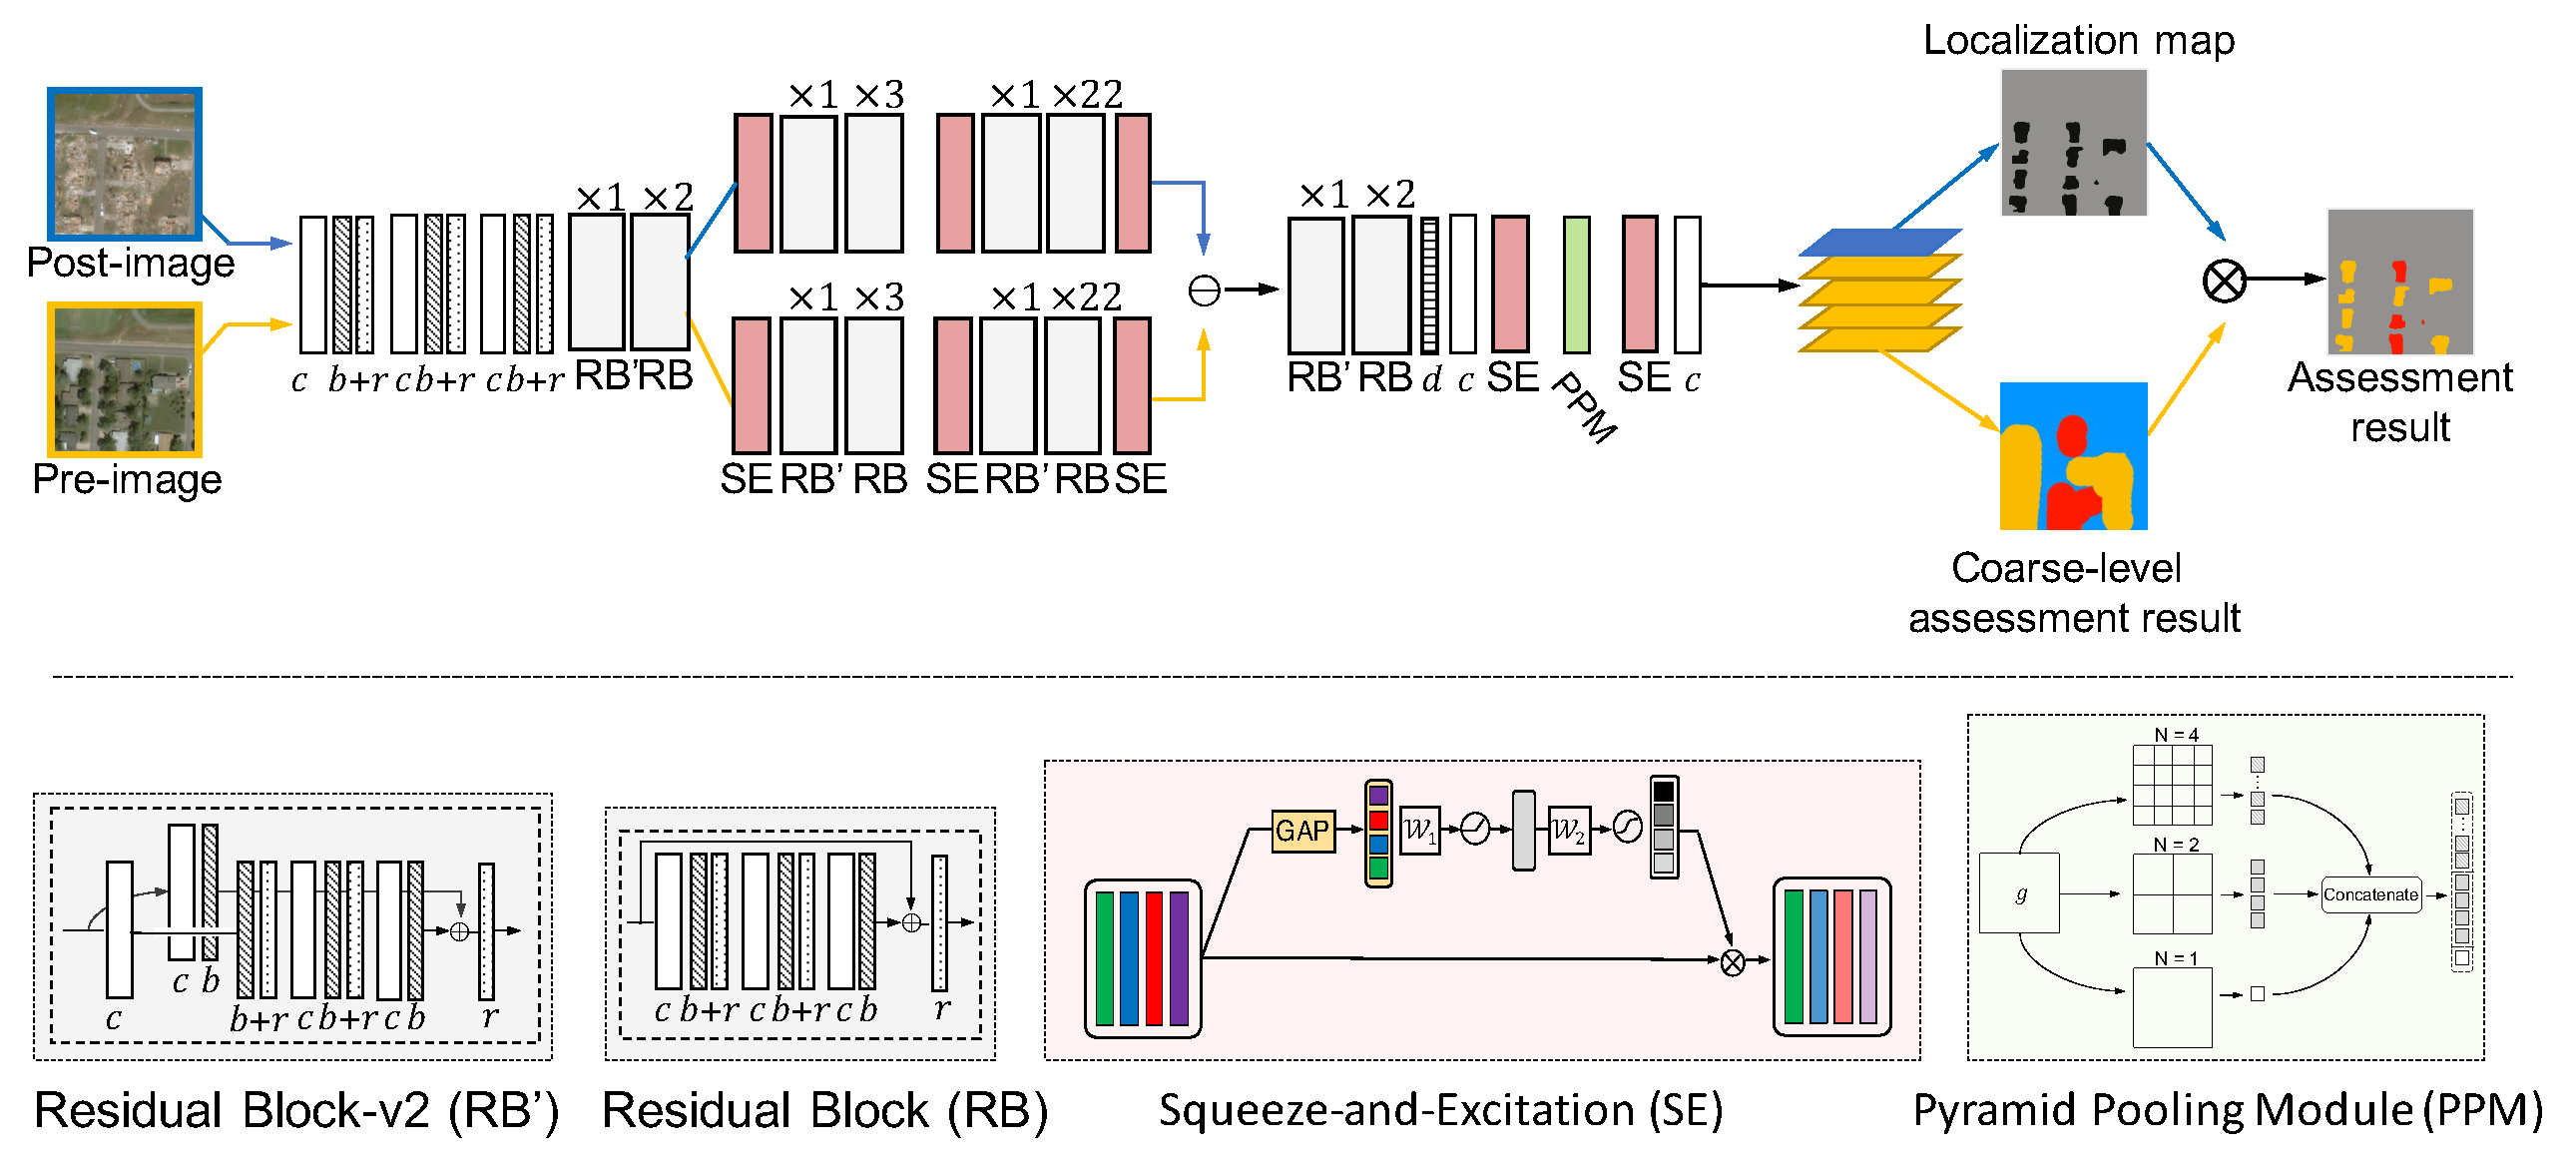
\includegraphics[width=\textwidth]{our_net.pdf}
    \caption{网络体系结构}
\end{figure}

本研究中构建的PPM-SSNet模型\cite{bai2020pyramid}采用扩张卷积、SE机制和PPM,详情如下。
建筑物损坏评估的任务分为两个阶段。第一阶段识别图像上的建筑物。这可以被视为一个定位问题,可以使用诸如CNN之类的系统来估计输入图像的二进制定位图。地图上带有1的位置表示该处为建筑物,地图上带有0的位置表示该处没有建筑物。然后,将定位图用作第二阶段的先验,对估计值等于1的位置进行损伤评估。基于这一思想,我们设计了一个网络来联合估计建筑物的位置并评估其损坏情况。我们单独使用灾前图像来估计位置图,然后使用灾前灾后图像来评估损失。为了利用定位图以产生准确的评估结果,我们直接将其乘以评估损失。这一过程修正了估计结果(见图1)。

图1展示了模型架构。我们让网络浅层的权重共享两个输入图像(即灾前/后图像),以便通过从这两个图像中共同学习低层特征来生成良好的“过滤器”库。随着层越来越深,我们不再共享权重,而是对两个输入使用独立的分支。这两个分支通过沿通道从另一个分支中减去一个来合并,有利于网络了解前后图像之间的差异。对于网络的尾部,我们使用层的一个分支来产生最终的估计结果。在网络中,我们使用了具有扩展卷积的RB结构和SE区块。网络可以根据RB中使用的扩张率提取特征,这可能会提高其估计的代表性。此外,SE块使得网络关注重要特征,同时抑制不太有用的特征。我们在网络的末端,即SE块之前使用PPM,并使用卷积层来聚合特征。






\subsubsection{缺失水域数据场景下多源数据协同的山洪监控}

\textbf{基准方法}

Zhang.\cite{zhang2021loss}利用径向基神经网络来对村庄、小镇等小流域区域进行损失预测。
Ouali.\cite{ouali2017fully}使用统计和机器学习方法研究水文变量 RFA 中与非线性相关的方面,使用人工神经网络 (ANN) 和广义加性模型 (GAM) 与基于非线性 ANN 的典型相关分析 (NLCCA) 程序相结合,以确保对所涉及的复杂过程进行适当的非线性建模。结果表明,完全非线性模型是最合适的。
Zhu.\cite{zhu2019hydrological}采用了八个大气环流模型(GCM)和两种基于人工智能的方法(支持向量回归、SVR和极限学习机(ELM))的集合,以建立对气候变化的历史径流响应,发现基于人工智能的SVR和ELM方法在预测未来水文响应方面表现出非常好的性能。结果还表明,在类似山区流域的局部区域模型性能更优。
Potdar.\cite{potdar2021toward}探讨了洪峰流量、降雨变异性和流域地形之间的一阶相关性,并使用多维统计建模方法揭示了这些复杂的相互作用。在不同的机器学习技术中,XGBoost用于通过变量重要性分析确定影响峰值流量的重要地形和降雨特征。创建了一个具有低偏差和方差的简约模型,可用于未来的山洪爆发预测。结果证实,尽管流域内降雨的空间组织对流域响应有重大影响,但流域地形是洪峰流量的主要驱动因素。
Ragettli.\cite{ragettli2017modeling}使用决策树学习来探索参数集在整个流域描述符空间中的可转移性,建立了中国十个省份35个集水区的半分布式降雨径流模型。在一系列遗漏测试中,评估了模型在假定无资料集水区检测洪水事件的能力。


\textbf{我们的方法}
% picked!
\cite{yang2020physical}物理分布水文模型在大型流域水文模拟中是有效的,但水文特征的复杂特性限制了其应用。为了在实践中有效地管理水资源,需要一个易于使用和高效的水文模型。基于机器学习(ML)的模型有可能提供气象预报和水文响应之间的快速映射路径,而无需详细描述相应的物理过程。然而,广泛的数据需求、对空间变异性的忽视以及极端流量的低性能限制了ML模型的应用。本研究试图通过将基于物理的分布式水文模型与人工神经网络(ANN)、计算机视觉(CV)和分类方法(CA)相结合,开发基于ML的水文模型。为了解决训练不足的问题,我们使用物理分布式水文模型(GBHM)和随机降雨发生器生成大量的合成数据(GBHM-ANN)。为了改进极端流模拟,我们在GBHM-ANN(GBHM-ANN-CA)中加入了分类方法。为了捕获预测因子的空间变异性,我们还使用基于局部二元模式的计算机视觉方法来形成GBHM-ANN-CA-CV模型。综合案例研究表明了这三种建模方法的有效性。最后,我们使用泰国湄南河上游盆地的真实数据评估GBHM-ANN-CA-CV。结果表明,在数据有限的流域,新的数据驱动模型的预测精度大大提高。具体而言,CV提取的空间信息可以提高数据驱动水文模型的鲁棒性,CA可以极大地改进高流量模拟。对于长期的日径流模拟,组合模型具有令人满意的精度。这项研究证明了基于ML的水文模型在水资源管理中的潜力,特别是在不断变化的环境中。


在本研究中,我们构建了一个物理过程和机器学习混合水文模型(GBHM-ANN-CA-CV)进行水文模拟,建模框架如图2所示。该模型主要由四个主要步骤组成。第一步是数据预处理,包括输入变量选择、训练数据生成和空间特征提取。由于该模型由GBHM生成的合成数据驱动,因此使用相同的输入。模型输入由三类变量组成,包括气象变量、植被参数和集水区地貌信息。气象输入包括通过Penman-Monteith方程计算的日降水量、日平均气温、日相对湿度和日潜在蒸散量。植被输入包括被线性插值为日分辨率的LAI。集水区地貌输入包括从DEM导出的坡度、坡度长度和高程信息。关于模型输入的详细信息见表2。确定模型输入后,使用SRG和GBHM生成用于模型开发的基于物理的合成数据。利用合成数据集,通过LBP-CV提取输入变量的空间特征,并将其串联形成ML的特征空间。为了避免模型过度拟合,我们采用主成分分析(PCA)进一步降低特征空间的维数。
\subsection{主要创新点}

从应用角度上看,我们的优势主要在:

本课题团队针对Google团队的HydroNet,结合国内数据进行调整,已经取得超越Google效果,构筑了国内特色的HydroNet,其核心更是使用了在AI领域一统NLP和CV的Transformer。结合基于强化学习+变分推断的山洪模拟的数据增强,在少量标注数据的情况下即可对无资料流域进行稳健预测,原理是采用迁移学习和半监督学习的方法,来借助全空间区域检测的遥感图像,以攫取有资料流域(Gauged Basins)的气象数据和水位信息。不仅仅对于无资料流域的预测有质的提升,其变分推断涉及的隐变量在深度学习的框架下引入统计学概率图模型不仅具有难得的解释力,对于任何形式的数据缺失都能够较好支撑。在知识蒸馏技术的帮助下,相比于Google团队,我们的HydroNet模型体积要小十倍,速度也要快十倍,对于快速监控和预测山洪有更好的时效性。建筑物级别的损失识别是我们团队的研究传统强项,可以在相关语义分割赛事中取得TOP3成绩。

从学术角度上看,我们的创新主要在:

1.整个课题所有解决方案均同时考虑深度结合水文模型和深度学习方法,保证鲁棒性、极端情况依旧稳定的条件下追求更高的性能。并未一味地追求模型的参数量,在深度学习的基础上引入变分推断的概率图,与传统统计模型、物理模型的原有工作有衔接、有发展。

2.对于无资料流域的数据,采用迁移学习和半监督学习的方法,来借助全空间区域检测的遥感图像,以攫取有资料流域(Gauged Basins)的气象数据和水位信息,方法上借鉴大量AI前沿方法。

3.对于遥感级别的数据处理使用像素级别的语义分割方法,使得损失评估能够达到建筑物级别的精细度,得益于预训练和迁移学习,我们的遥感模型在小规模图像上也具备很好的信息提取能力。




\subsection{研究计划及预期进展}
(包括研究进度计划及阶段目标)

\subsection{预期研究成果和考核指标}
(含预期产生的专利、著作、技术方法、软件产品等,须具体、明确、可考核)




\section{研究基础}

\subsection{与申请课题有关的研究工作基础和已取得成绩}
(包括已经取得的知识产权,如专利、著作、技术秘密等)

\subsection{现有研究条件情况}

\subsection{申请者和主要成员研究工作简历}
(包括近期承担与本课题有关的预研项目、基金项目和其它项目情况,及发表论著目录等)




\bibliographystyle{plain}
\bibliography{paper.bib}

\end{document}